\documentclass{article}

\usepackage{hyperref}
\hypersetup{
	colorlinks=true,
	linkcolor=blue,
	urlcolor=cyan,}
\usepackage{booktabs}
\usepackage{textgreek}

%%%%%%%%%%%%%%%%%%%%%%%%%%%%%%%%%%%%%%%%%
% Lachaise Assignment
% Structure Specification File
% Version 1.0 (26/6/2018)
%
% This template originates from:
% http://www.LaTeXTemplates.com
%
% Authors:
% Marion Lachaise & François Févotte
% Vel (vel@LaTeXTemplates.com)
%
% License:
% CC BY-NC-SA 3.0 (http://creativecommons.org/licenses/by-nc-sa/3.0/)
% 
%%%%%%%%%%%%%%%%%%%%%%%%%%%%%%%%%%%%%%%%%

%----------------------------------------------------------------------------------------
%	PACKAGES AND OTHER DOCUMENT CONFIGURATIONS
%----------------------------------------------------------------------------------------

\usepackage{amsmath,amsfonts,stmaryrd,amssymb} % Math packages

\usepackage{enumerate} % Custom item numbers for enumerations

\usepackage[ruled]{algorithm2e} % Algorithms

\usepackage[framemethod=tikz]{mdframed} % Allows defining custom boxed/framed environments

\usepackage{listings} % File listings, with syntax highlighting
\lstset{
	basicstyle=\ttfamily, % Typeset listings in monospace font
}

%----------------------------------------------------------------------------------------
%	DOCUMENT MARGINS
%----------------------------------------------------------------------------------------

\usepackage{geometry} % Required for adjusting page dimensions and margins

\geometry{
	paper=a4paper, % Paper size, change to letterpaper for US letter size
	top=2.5cm, % Top margin
	bottom=3cm, % Bottom margin
	left=2.5cm, % Left margin
	right=2.5cm, % Right margin
	headheight=14pt, % Header height
	footskip=1.5cm, % Space from the bottom margin to the baseline of the footer
	headsep=1.2cm, % Space from the top margin to the baseline of the header
	%showframe, % Uncomment to show how the type block is set on the page
}

%----------------------------------------------------------------------------------------
%	FONTS
%----------------------------------------------------------------------------------------

\usepackage[utf8]{inputenc} % Required for inputting international characters
\usepackage[T1]{fontenc} % Output font encoding for international characters

\usepackage{XCharter} % Use the XCharter fonts

%----------------------------------------------------------------------------------------
%	COMMAND LINE ENVIRONMENT
%----------------------------------------------------------------------------------------

% Usage:
% \begin{commandline}
%	\begin{verbatim}
%		$ ls
%		
%		Applications	Desktop	...
%	\end{verbatim}
% \end{commandline}

\mdfdefinestyle{commandline}{
	leftmargin=10pt,
	rightmargin=10pt,
	innerleftmargin=15pt,
	middlelinecolor=black!50!white,
	middlelinewidth=2pt,
	frametitlerule=false,
	backgroundcolor=black!5!white,
	frametitle={Command Line},
	frametitlefont={\normalfont\sffamily\color{white}\hspace{-1em}},
	frametitlebackgroundcolor=black!50!white,
	nobreak,
}

% Define a custom environment for command-line snapshots
\newenvironment{commandline}{
	\medskip
	\begin{mdframed}[style=commandline]
}{
	\end{mdframed}
	\medskip
}

%----------------------------------------------------------------------------------------
%	FILE CONTENTS ENVIRONMENT
%----------------------------------------------------------------------------------------

% Usage:
% \begin{file}[optional filename, defaults to "File"]
%	File contents, for example, with a listings environment
% \end{file}

\mdfdefinestyle{file}{
	innertopmargin=1.6\baselineskip,
	innerbottommargin=0.8\baselineskip,
	topline=false, bottomline=false,
	leftline=false, rightline=false,
	leftmargin=2cm,
	rightmargin=2cm,
	singleextra={%
		\draw[fill=black!10!white](P)++(0,-1.2em)rectangle(P-|O);
		\node[anchor=north west]
		at(P-|O){\ttfamily\mdfilename};
		%
		\def\l{3em}
		\draw(O-|P)++(-\l,0)--++(\l,\l)--(P)--(P-|O)--(O)--cycle;
		\draw(O-|P)++(-\l,0)--++(0,\l)--++(\l,0);
	},
	nobreak,
}

% Define a custom environment for file contents
\newenvironment{file}[1][File]{ % Set the default filename to "File"
	\medskip
	\newcommand{\mdfilename}{#1}
	\begin{mdframed}[style=file]
}{
	\end{mdframed}
	\medskip
}

%----------------------------------------------------------------------------------------
%	NUMBERED QUESTIONS ENVIRONMENT
%----------------------------------------------------------------------------------------

% Usage:
% \begin{question}[optional title]
%	Question contents
% \end{question}

\mdfdefinestyle{question}{
	innertopmargin=1.2\baselineskip,
	innerbottommargin=0.8\baselineskip,
	roundcorner=5pt,
	nobreak,
	singleextra={%
		\draw(P-|O)node[xshift=1em,anchor=west,fill=white,draw,rounded corners=5pt]{%
		Question \theQuestion\questionTitle};
	},
}

\newcounter{Question} % Stores the current question number that gets iterated with each new question

% Define a custom environment for numbered questions
\newenvironment{question}[1][\unskip]{
	\bigskip
	\stepcounter{Question}
	\newcommand{\questionTitle}{~#1}
	\begin{mdframed}[style=question]
}{
	\end{mdframed}
	\medskip
}

%----------------------------------------------------------------------------------------
%	WARNING TEXT ENVIRONMENT
%----------------------------------------------------------------------------------------

% Usage:
% \begin{warn}[optional title, defaults to "Warning:"]
%	Contents
% \end{warn}

\mdfdefinestyle{warning}{
	topline=false, bottomline=false,
	leftline=false, rightline=false,
	nobreak,
	singleextra={%
		\draw(P-|O)++(-0.5em,0)node(tmp1){};
		\draw(P-|O)++(0.5em,0)node(tmp2){};
		\fill[black,rotate around={45:(P-|O)}](tmp1)rectangle(tmp2);
		\node at(P-|O){\color{white}\scriptsize\bf !};
		\draw[very thick](P-|O)++(0,-1em)--(O);%--(O-|P);
	}
}

% Define a custom environment for warning text
\newenvironment{warn}[1][Warning:]{ % Set the default warning to "Warning:"
	\medskip
	\begin{mdframed}[style=warning]
		\noindent{\textbf{#1}}
}{
	\end{mdframed}
}

%----------------------------------------------------------------------------------------
%	INFORMATION ENVIRONMENT
%----------------------------------------------------------------------------------------

% Usage:
% \begin{info}[optional title, defaults to "Info:"]
% 	contents
% 	\end{info}

\mdfdefinestyle{info}{%
	topline=false, bottomline=false,
	leftline=false, rightline=false,
	nobreak,
	singleextra={%
		\fill[black](P-|O)circle[radius=0.4em];
		\node at(P-|O){\color{white}\scriptsize\bf i};
		\draw[very thick](P-|O)++(0,-0.8em)--(O);%--(O-|P);
	}
}

% Define a custom environment for information
\newenvironment{info}[1][Info:]{ % Set the default title to "Info:"
	\medskip
	\begin{mdframed}[style=info]
		\noindent{\textbf{#1}}
}{
	\end{mdframed}
}
 % Include the file specifying the document structure and custom commands

%----------------------------------------------------------------------------------------
%	ASSIGNMENT INFORMATION
%----------------------------------------------------------------------------------------

\title{Week 4: Electroencephalography (EEG)}
\author{BIOE 320 Systems Physiology Laboratory} 
\date{}
%----------------------------------------------------------------------------------------

\begin{document}
\large
\maketitle

\section*{Objectives}
\begin{enumerate}
	\item To record an EEG from an awake, resting subject under the following conditions:
	\begin{itemize}
		\item Relaxed, eyes open
		\item Relaxed, eyes closed
		\item Mental arithmetic
		\item Hyperventilation
	\end{itemize}
	\item To examine alpha, beta, delta, and theta components of the EEF complex
\end{enumerate}

\section*{Background}
The brain is encased by the cranium and protected by a thin layer of skin, the scalp. The cerebral cortex is the largest part of the brain that lies underneath the cranium. The cerebral cortex is responsible for many major functions and is involved in sensing and processing various types of information. It consists of four different lobes: the frontal, parietal, occipital, and temporal (Fig. \ref{brain}). The front lobe of the cortex controls voluntary muscle contractions, the occipital lobe processes visual information, the temporal lobe processes auditory information, and the parietal lobe processes other somatosensory information.

\begin{figure}[h]
\centering
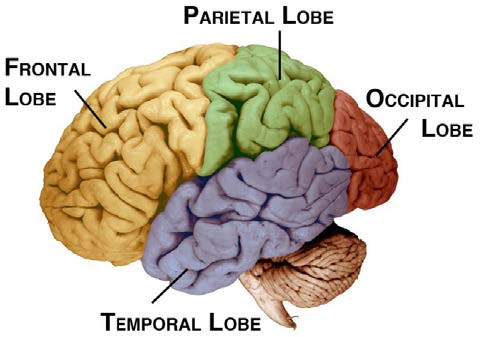
\includegraphics[width=0.5\textwidth]{../images/EEG_1.jpg}	
\caption{Function of muscle spindle during a monosynaptic stretch reflex.}
\label{brain}
\end{figure}

The brain is always electrically active, even when asleep, as nerve impulses are always being sent to and from cortical neurons. Electrodes placed on the scalp can measure patterns of electrical activity as a series of complex waveforms, called an electroencephalogram, or EEG. The firing of neurons must occur synchronously in order to be detected, so the intensity of brain waves, which are neuronal electrical impulses that travel through the brain (Fig. \ref{brainwaves}, is determined by the synchrony of the firing neurons, not by the total electrical activity.

\begin{figure}[h]
\centering
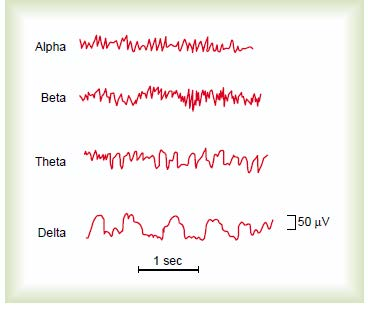
\includegraphics[width=0.6\textwidth]{../images/EEG_2.jpg}	
\caption{Different types of brain waves in an example EEG}
\label{brainwaves}
\end{figure}

In an EEG, the electrodes attached to the scalp measure the difference in electric potential (voltage) in the different lobes of the brain. In this lab, we will place the electrodes using a standard bipolar method. In a bipolar recording, the voltage difference between two electrodes placed over the cortical region of interest is measured with respect to a third reference electrode. This will be elaborated in the protocol.

\subsection*{Types of Brain Waves}
\subsubsection*{Alpha Waves: 8-13 Hz}
Alpha waves are the most common wave pattern for adults in an awake but relaxed state with their eyes closed. Alpha waves of the largest amplitude are usually measured from the occipital and parietal lobes. Biological females have higher mean frequencies of alpha waves than biological males. Alpha waves also diminish when the subject opens their eyes and is alert to external stimuli.

\subsubsection*{Beta Waves: 13-20 Hz}
Beta waves occur when the subject is alert, attentive to external stimuli, or exerting mental effort. It also occurs during rapid eye movement (REM) when the person is sleeping. Beta waves have lower amplitude than alpha waves, indicating that destructive interference or desynchronization occurs. Instead of regular sinusoidal patterns, positive and negative portions of different waves start to overlap and cancel each other out, resulting in the lower amplitude observed. Beta waves are best recorded from the frontal lobes.

\subsubsection*{Theta Waves: 5-8 Hz}
Theta waves are low frequency waves that increase during non-RE sleep. They occur as people transition from lighter to deeper states of sleep and can be best measured from the temporal and occipital lobes. Theta waves also occur for brief periods of time when the subject is frustrated. They can also be seen in awake newborn infants.

\subsubsection*{Delta Waves: 1-5 Hz}
Delta waves are the lowest frequency rhythms observed in an EEG. They can be seen during the period right before the deepest stage of sleep or in awake subjects when they undergo difficult mental activity. They are best recorded from the cerebral cortex and can also be present in awake infants.\\

\textit{Synchrony} occurs when neurons fire at the same time. When the neurons fire at the same time, they constructively interfere with each other and as a result, larger EEG waves can be seen. For this lab it is important to understand the concept of destructive interference of waves, in which the overall wave amplitude is lowered when the positive and negative portions of the two different waves cancel each other out. Therefore, the amplitude of the waves measured in the EEG depends on the number of neurons firing in synchrony rather than overall electrical activity. An example of this phenomenon is \textit{alpha block}, where a new waveform interferes with alpha waves, leading to a decrease in the amplitude of the EEG recording (Fig. \ref{alphablock}).

\begin{figure}[h]
\centering
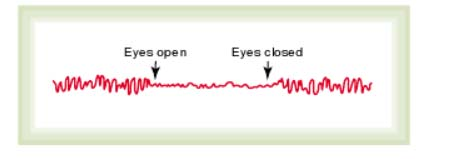
\includegraphics[width=0.6\textwidth]{../images/EEG_3.jpg}	
\caption{An example of alpha block}
\label{alphablock}
\end{figure}

\section*{Required Supplies}
\begin{itemize}
	\item BIOPAC student labs lesson L03: EEG 1 and L04: EEG 2
	\item BIOPAC MP3X data acquisition unit
	\item BIOPAC electrode lead set
	\item BIOPAC reflex hammer transducer (SS36L)
	\item BIOPAC disposable vinyl electrodes (3 per subject)
	\item Elastic headband or cap to hold electrodes against the scalp
	\item Yoga mat (optional)
	\item Optional but useful: alcohol wipes, abrasive pads, physiology tape, electrode gel
\end{itemize}

\section*{Setting Up for Experiment 1}
\begin{enumerate}
	\item Turn on the MP3X acquisition unit by flipping the switch found on the back panel
	\item Launch the BIOPAC software by clicking on the BSL lessons 3.7.6 icon that can be found on your desktop. Select L03-EEG-1 as shown in Fig. \ref{lesson}.
		\begin{figure}[h]
		\centering
	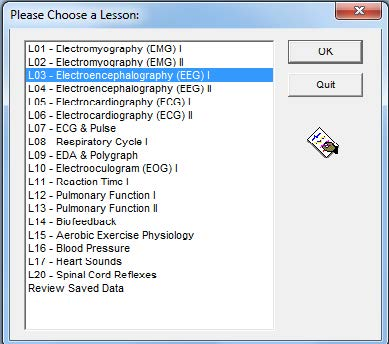
\includegraphics[width=0.6\textwidth]{../images/EEG_4.jpg}	
		\caption{Selecting BIOPAC lesson L03}
		\label{lesson}
		\end{figure}

	\item When the prompt asking for your file name appears, name the file using your name and a description about the lab. The BIOPAC student software will create a folder inside of the BIOPAC Student Lab folder where all your data will be stored.
	\item Plug the electrode lead set into channel 1 of the MP3X unit.
	\item Select a subject for the EEG and have them assume a relaxed position. Move as much hair as possible away from the adhesion area and apply pressure to the electrodes for about a minute to maximize adhesion.
	\item Place two electrodes on the scalp and one on the earlobe (ground) as seen in Fig. \ref{electrodes}.
		\begin{itemize}
			\item Red (+): highest placed electrode
			\item White (-): electrode behind ear
			\item Black (ground): earlobe
		\end{itemize}
		
		 \begin{figure}[h]
	\centering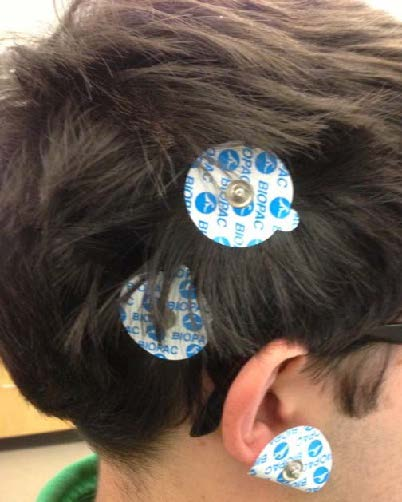
\includegraphics[width=0.35\textwidth]{../images/EEG_5a.jpg}
	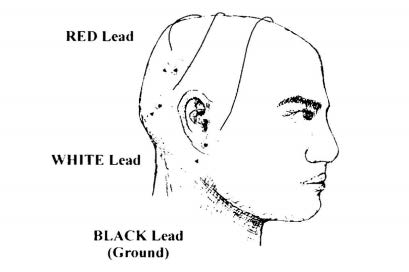
\includegraphics[width=0.6\textwidth]{../images/EEG_5b.jpg}		
		\caption{Proper electrode placement}
		\label{electrodes}
		\end{figure}
		
	\item Secure the electrodes by wearing a swim cap or a headband over the electrodes to keep them in place. Proper electrode contact is really important for this lab, so make sure that your electrodes are properly attached before placing the swim cap/headband over them.\\
	
		Some tips for achieving the best data:
		\begin{itemize}
			\item Be sure to separate the hair so the electrode has maximum surface area contact with the scalp.
			\item Apply pressure to the electrodes for about 1 minute after initial placement to make them secure. Do not immediately connect the leads.
			\item Make sure the subject is in a relaxed position (in a chair or lying down on a yoga mat).
			\item Subject should remain as still as possible since blinking and other movements will affect the recording of all the brain rhythms and interfere with the data.
			\item Putting a swim cap or headband on will secure the leads with constant pressure. Have the subject hold the swim cap to their forehead, while a second person pulls the swim cap carefully over the rest of the head.
			\item Make sure the electrode leads are not being pulled on.
		\end{itemize}
\end{enumerate}

\section*{Calibration}
\begin{enumerate}
	\item Check to make sure the electrodes are secure and the lead is plugged into channel 1.
	\item The calibrate button is in the upper left corner of the setup window. Click the calibrate button and the procedure will begin. It will stop automatically after 8 seconds. After the 8 second calibration period, the screen should look like Fig. \ref{calibration}.
	
		\begin{figure}[h]
	\centering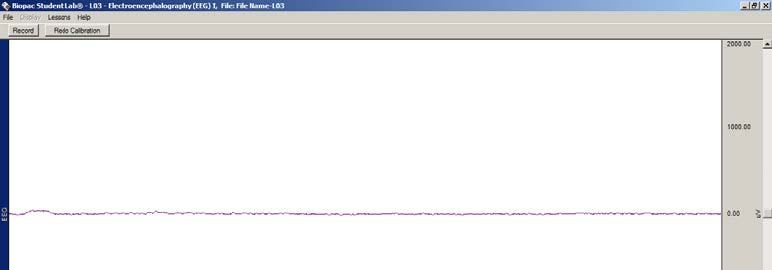
\includegraphics[width=0.6\textwidth]{../images/EEG_6a.jpg}
	\centering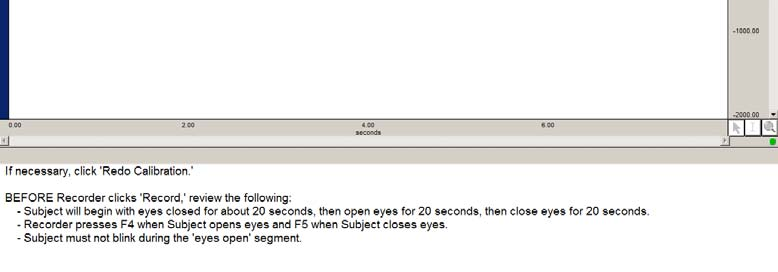
\includegraphics[width=0.6\textwidth]{../images/EEG_6b.jpg}	
		\caption{Calibration screen after the 8 second recording}
		\label{calibration}
		\end{figure}
	
	\item If the data shows any large spikes or is significantly different from Fig. \ref{calibration}, redo the calibration by clicking the Redo Calibration button.
\end{enumerate}

\section*{Data Acquisition}
You will record the raw EEG signal while the subject is relaxed with their eyes closed, eyes opened, and then eyes closed again for a time interval. After recording the EEG, the data for the four different brain rhythms will be analyzed.\\

Before continuing:
\begin{enumerate}
	\item Make sure the electrodes still have good contact and are not moving around.
	\item Make sure the subject is staying still (including the facial muscles).
	\item It might help if the subject tries to focus on breathing slowly to help them relax.
\end{enumerate}

\begin{enumerate}
	\item Click Record, and the first segment marker will be inserted.
	\item The subject should keep their eyes closed for 10 seconds.
	\item After 10 seconds, insert a data marker and tell the subject to open their eyes.
	\item The subject should keep their eyes open for 10 seconds, trying not to blink. They should also look around at different things to stimulate the brain.
	\item After 10 seconds of keeping their eyes open, insert another data marker and tell the subject to close their eyes for 10 seconds again.
	\item After this third interval of 10 seconds, stop the recording by clicking Stop.
	\item The data should look like Fig. \ref{eyes}. If it looks similar to the figure, proceed to the next step. If it looks significantly different, redo the data collection.
	\begin{warn}
		If you click redo, you will lose the data that was just recorded.
	\end{warn}
	
	\item If the data is good, click Done, and a dialog box will ask if you are finished. Click "yes" to end the data recording and save the data.
	\item Select "analyze current data file" from the next dialog box, and you should see four different graphs with each of the brain waves (alpha, beta, delta, and theta) displayed. If you would like to record this data again, click the Redo button.
	\item Do not remove the electrodes yet, as you will need them for the next experiment.
\end{enumerate}

\section*{Data Analysis}
\begin{enumerate}
	\item Make sure the channel number designations are as follows:
		\begin{itemize}
			\item channel 1: EEG
			\item channel 40: alpha
			\item channel 41: beta
			\item channel 42: delta
			\item channel 43: theta
		\end{itemize}
		
	\item Set up the measurement boxes as follows:\begin{itemize}
		\item channel 40: stddev
		\item channel 41: stddev
		\item channel 42: stddev
		\item channel 43: stddev
	\end{itemize}
	
	\item Use the I-beam tool to obtain the data you need for your handout.
	\item What information does using the computed value of the standard deviation of the amplitude give you as compared to other statistical measurements such as the mean of the amplitude?
	\begin{info}
		\textit{Freq} converts the time segment of the selected region into a frequency in cycles/second. You must be careful to select an area that contains only one cycle of the wave.
	\end{info}
	
	\item Zoom in to displace 3-4 seconds of data during the first 10 seconds of eyes closed by clicking on the magnifying glass icon in the bottom right corner and clicking on the graph where you would like to zoom in.
	\item Using the I-beam selection tool, select a representative alpha waveform to complete the second table in your handout.
	\item Repeat for two other alpha wave cycles.
	\item Repeat steps 5 and 6 for the remaining types of waves: beta, delta, and theta.
	\item Save the data file.
	\item Are the frequencies within the range of expected, published values?
	\item Examine the alpha and beta waveforms for change between the "eyes closed" and "eyes open" states. Does desynchronization of the alpha rhythm occur when the eyes are open? Explain.
	\item Does the beta rhythm become more pronounced in the "eyes open" state?
	\item Examine the delta and theta rhythms. Is there an increase, decrease, or no change in the delta and theta activity when the eyes are open? Explain your observations.
	\item Could you see evidence of synchrony and/or alpha block in your EEG measurements? Explain.
\end{enumerate}

\section*{Setting Up for Experiment 2}
\begin{enumerate}
	\item Keep the setup the same as in the first experiment and make sure the electrodes are still secure to the subject.
	\item Open BSL lesson L04-EEG-2.
	\item Prepare the subject by having them either sit in a chair or lie down on a yoga mat. They should be relaxed with their eyes closed. Throughout the experiment, you will need to insert markers to separate the segments.
\end{enumerate}

\section*{Data Acquisition}
Be sure to read all of the instructions before beginning any data collection.

Tips for successful data collection:
\begin{itemize}
	\item Try not to blink during the eyes open segment.
	\item The subject should not talk out loud during any of the recordings.
	\item Try to focus on breathing slowly and relaxing for the eyes closed segments.
	\item During the mental math section, make sure the subject is challenged and doing math the entire time, but do not make it too challenging that they give up on the problem. A good way to do it is by giving the subject double digit numbers to add.
	\item Make sure the subject is not still hyperventilating during the recovery section.
\end{itemize}

\subsection*{Segment 1: Eyes Closed}
\begin{enumerate}
	\item Click Record. The subject should have their eyes closed and be relaxed for 10 seconds. After 10 seconds, click Suspend.
\end{enumerate}

\subsection*{Segment 2: Performing Arithmetic}
\begin{enumerate}
	\item The lab partner who is not connected to the electrodes should verbally tell the subject a set of mental math problems while the subject remains relaxed with their eyes closed.
	\item Record this segment for 20 seconds. After 20 seconds, click Suspend.
\end{enumerate}

\subsection*{Segment 3: Hyperventilation}
\begin{enumerate}
	\item The lab partner who is not connected to the electrodes should now instruct the subject to hyperventilate for 2 minutes while the subject has their eyes closed.\begin{warn}
		Stop the procedure if the subject feels sick or dizzy.
	\end{warn}
	
	\item At the end of the 2 minute period, click Resume. Do this as fast as possible.
	\item Record for 10 seconds while the subject is recovering from hyperventilation. During this time, the subject should be in a relaxed state with their eyes closed.
	\item After 10 seconds, click Suspend.
\end{enumerate}

\subsection*{Section 4: Eyes Open}
\begin{enumerate}
	\item The lab partner who is not connected to the electrodes should instruct the subject to open their eyes and remain relaxed.
	\item Clock on Resume and record for 10 seconds.
	\item After 10 seconds, click Suspend.
	\item When you are ready to review your data, click "Done" and save your data. You may now remove the electrode cables and peel off the electrodes.
\end{enumerate}

\section*{Data Analysis}
\begin{enumerate}
	\item Mark the channel numbers as follows:\begin{itemize}
		\item channel 1: raw EEG
		\item channel 40: alpha rhythm
		\item channel 41: alpha RMS
	\end{itemize}
	
	\item Set up the measurement boxes as follows:\begin{itemize}
		\item channel 1: stddev
		\item channel 40 stddev
		\item channel 41: mean
		\item channel 40: freq
	\end{itemize}
	
	\item Use the I-Beam tool to analyze the data you need to complete the table in your handout.
	\item Under what conditions where the alpha wave amplitudes highest? Why?
	\item How did the level of concentration (focused thinking) affect the data?
	\item What kind of differences would you expect when measuring the amplitude of alpha and beta waves recorded from a subject tested alone in a darkened room and a subject tested in a lab full of students? Justify.
\end{enumerate}

\begin{info}
	Export data from Segment 1 (eyes open) and Segment 3 (hyperventilation). You will need these values to complete your post-lab assignment.
\end{info}
\end{document}
